\documentclass[grad]{ontariotechu-thesis}
\usepackage{lipsum} 
\usepackage{changepage}
\usepackage{setspace}
\usepackage{multicol}
\usepackage{graphicx}
\usepackage[export]{adjustbox}
\usepackage{subcaption}
\usepackage{rotating}
\usepackage{footnote}
\usepackage{caption}
\usepackage{amsmath,amssymb}
\usepackage{algorithm}
\usepackage{listings}
\usepackage[noend]{algpseudocode}
\usepackage[shortcuts]{extdash}
\usepackage{ctable}
\usepackage{dcolumn}
\usepackage{multirow}
\usepackage{color}
\usepackage{tcolorbox}

\definecolor{codegreen}{rgb}{0,0.6,0}
\definecolor{codegray}{rgb}{0.5,0.5,0.5}
\definecolor{codepurple}{rgb}{0.58,0,0.82}
\definecolor{backcolour}{rgb}{0.95,0.95,0.92}

\usepackage{listings}
\usepackage{xcolor}

\definecolor{codegray}{gray}{0.95}
\definecolor{keywordcolor}{rgb}{0.3,0.3,0.8}

\usepackage{amsthm}
\newtheorem{definition}{Definition}

\usepackage{graphicx} % in the preamble

\usepackage{color}
\usepackage{listings}
\usepackage{xcolor}

\lstset{
	language=Python,
	basicstyle=\ttfamily\footnotesize,
	keywordstyle=\color{blue},
	commentstyle=\color{gray},
	stringstyle=\color{teal},
	showstringspaces=false,
	breaklines=true,
	frame=single
}

\lstset{
	backgroundcolor=\color{codegray},
	basicstyle=\ttfamily\small,
	keywordstyle=\color{keywordcolor}\bfseries,
	commentstyle=\color{gray},
	stringstyle=\color{red},
	numbers=left,
	numberstyle=\tiny\color{gray},
	stepnumber=1,
	numbersep=5pt,
	showspaces=false,
	showstringspaces=false,
	showtabs=false,
	frame=single,
	breaklines=true,
	captionpos=b,
	language=Python
}


\lstdefinestyle{mystyle}{
    backgroundcolor=\color{backcolour},   
    commentstyle=\color{codegreen},
    keywordstyle=\color{magenta},
    numberstyle=\tiny\color{codegray},
    stringstyle=\color{codepurple},
    basicstyle=\footnotesize,
    breakatwhitespace=false,         
    breaklines=true,                 
    captionpos=b,                    
    keepspaces=false,                 
    numbers=left,                    
    numbersep=5pt,                  
    showspaces=false,                
    showstringspaces=false,
    showtabs=false,                  
    tabsize=2
}
\lstset{style=mystyle}

\DeclareMathOperator*{\argmax}{arg\,max}
\DeclareMathOperator*{\argmin}{arg\,min}
\DeclareMathOperator{\E}{\mathbb{E}}
\newcommand{\pluseq}{\mathrel{+}=}
\newcommand{\minus}{\scalebox{0.3}[0.5]{$-$}}
\newcommand\todo[1]{\textcolor{red}{#1}}

\degree{Masters of Science} % Only used when grad option is chosen
\department{Computer Science}
%\faculty{Science}
%\gradyear{2020}
%\supervisor{Dr.~A.~Foo and Dr.~B.~Boo}
\author{Hafiz A. Amjad}
\title{In The World Of Deep Learning}
%\setcounter{tocdepth}{2}

\begin{document}
\begin{preliminary}

\maketitle

%\cleardoublepage
%\addcontentsline{toc}{chapter}{Certificate of Approval}
%\noindent \textcolor{red}{The University of Ontario Institute of Technology requires the
%Certificate of Approval (CoA) to be included as page %(ii) of
%the PRINTED version. Check the source file on how to add
%the provided CoA to your thesis.}

%\addcontentsline{toc}{chapter}{Abstract}
%\begin{abstract}
%  \lipsum[1]\\
%  \textcolor{red}{{\bf At most 150 words for Honors %Thesis/M.Sc. or 350 words for Ph.D.}}
%\vfill
%\noindent {\textbf{Keywords: } \space keyword1; %keyword2; keyword3; keyword4; keyword5}
%\end{abstract}


% \addcontentsline{toc}{chapter}{Dedication}
% \begin{dedication}
% ***   Put your Dedication here.   ***

% \lipsum[2]
% \end{dedication}
%\addcontentsline{toc}{chapter}{Acknowledgment}
%\begin{acknowledgements}
%***   Put your Acknowledgements here.   ***

%\lipsum[2]
%\end{acknowledgements}


\tableofcontents


\listoftables


\listoffigures


\end{preliminary}

\chapter{Philosophical Insights of Vector Spaces}
\section{Understanding Closure in \(\mathbb{R}^n\): Why Vector Spaces Are Chosen for Image Representation}

A vector space is a mathematical structure consisting of a set of  vectors that support two key operations: vector addition and scalar multiplication. These operations must satisfy a list of specific axioms—such as associativity, distributivity, and most importantly for our discussion, \emph{closure}. The space \(\mathbb{R}^n\), for instance, is the set of all \(n\)-dimensional vectors whose components are real numbers:
\[
x = \begin{bmatrix} x_1 \\ x_2 \\ \cdots \\ x_n \end{bmatrix}, \quad \text{where each } x_i \in \mathbb{R}.
\]
This makes \(\mathbb{R}^n\) an example of a real vector space.

\subsection{Meaning of Closure}
Closure under addition and scalar multiplication means that for any two vectors \( u, v \in \mathbb{R}^n \), their sum \( u + v \in \mathbb{R}^n \), and for any scalar \( a \in \mathbb{R} \), the scaled vector \( a u \in \mathbb{R}^n \). 

\subsection{Why Closure Matters for Images}
When an image is represented as a vector (for instance, flattening pixel intensities into an \(n\)-dimensional vector), we often wish to apply operations such as blending two images or adjusting brightness. These correspond respectively to vector addition and scalar multiplication. To ensure the result of these operations remains a valid image, we need the underlying representation space to be closed under these operations. Vector spaces like \(\mathbb{R}^n\) give us this guarantee by design.

\subsection{How \(\mathbb{R}^n\) Ensures Closure}
The structure of \(\mathbb{R}^n\) is built component-wise from the real numbers, and real numbers themselves are closed under addition and multiplication. That is:
\[
(x_1, \dots, x_n) + (y_1, \dots, y_n) = (x_1 + y_1, \dots, x_n + y_n),
\]
\[
a \cdot (x_1, \dots, x_n) = (a x_1, \dots, a x_n),
\]
where each operation is closed within \(\mathbb{R}\). Therefore, every result remains inside \(\mathbb{R}^n\).

Thus, when we say that \emph{“we are choosing to represent images in a space that is already structured to ensure closure,”} we mean that the vector space \(\mathbb{R}^n\) is not arbitrarily chosen. It is selected because it is algebraically and geometrically equipped with properties that make mathematical operations on images consistent, safe, and computationally tractable. Closure is one of the fundamental pillars of this structure.

\section{Understanding Column Space and Its Relevance in Deep Learning}

Linear algebra introduces the notion of a \textit{vector space} as a fundamental structure in which vectors can be added and scaled while remaining within the same space. Once, one understands that a space is defined by its basis vectors, the next conceptual step is to understand how specific types of subspaces emerge from matrices. One such subspace, central to both theoretical and applied linear algebra, is the \textit{column space}.

The term ``column space'' arises from a natural and practical consideration. When a matrix $A$ acts on a vector $x$ through multiplication ($Ax$), the result is a linear combination of the columns of $A$. That is, each element in the vector $x$ serves as a coefficient that scales one of the columns of $A$, and the final output is the sum of these scaled columns. Therefore, the set of all possible outputs that can be generated by multiplying $A$ with any vector $x$ forms a space—specifically, the \textit{space spanned by the columns of $A$}. This is precisely why it is called the column space: it is the image (or range) of the transformation defined by $A$, and that image is built solely from combinations of its columns.

The concept of column space is not merely a theoretical construction; it plays a pivotal role in determining the behavior and capacity of models in machine learning, particularly in deep learning. Consider a linear transformation implemented by a weight matrix $W$ within a neural network layer. The output of this layer, for any input vector $x$, is $Wx$, which lies entirely within the column space of $W$. No matter how complex the input data is, the transformation cannot produce an output vector outside of the column space. This reveals a critical limitation: if the column space is low-dimensional due to dependent columns (i.e., $W$ has low rank), then the layer has a limited capacity to represent diverse outputs. Such a situation can lead to underfitting, where the model fails to capture the complexity of the data.

Moreover, when designing autoencoders or dimensionality-reducing architectures such as bottleneck networks, the encoder's weight matrix defines a lower-dimensional subspace where input data is projected. This subspace is none other than the column space of the encoder matrix. The success of such models depends on how well this column space captures the essential structure of the input data. If the column space misses important directions, then crucial information is irretrievably lost during encoding.

Even in unsupervised methods like Principal Component Analysis (PCA), the reduced representation of data is achieved by projecting it onto the column space of the principal component matrix. Thus, the quality of dimensionality reduction is inherently tied to how well the column space aligns with the intrinsic geometry of the data distribution.

Furthermore, during the initialization of deep networks, care is taken to ensure that the initial weight matrices span a sufficiently rich column space. Initialization methods such as Xavier or orthogonal initialization aim to create column spaces that are isotropic and well-distributed, allowing gradients to propagate effectively and models to explore a wide range of outputs early in training.

In conclusion, while the term ``space'' might initially evoke an abstract mathematical landscape, the specification of ``column space'' grounds this abstraction in the practical mechanics of linear transformations. It denotes the exact set of outputs a matrix can produce and, in doing so, highlights the expressive boundaries of models in deep learning. Understanding column space equips one with the tools to reason about capacity, compression, and learnability in neural architectures.

\chapter{Natural Language Processing}
\section{\texttt{vectorizer.fit\_transform}}

In machine learning (especially in Natural Language Processing), we often use 
\textbf{vectorizers} from libraries like \textbf{scikit-learn}, such as 
\texttt{CountVectorizer} and \texttt{TfidfVectorizer}. 
These convert text (words, sentences, documents) into \textbf{numerical vectors} 
that models can understand. 

When you call \texttt{fit}, the vectorizer learns the vocabulary from your training data:

\begin{lstlisting}[caption=Learning the vocabulary with \texttt{fit}]
	from sklearn.feature_extraction.text import CountVectorizer
	
	vectorizer = CountVectorizer()
	vectorizer.fit(["I Love NLP", "I Love Python"])
\end{lstlisting}

This produces the learned dictionary (vocabulary):

\begin{lstlisting}[caption=Vocabulary learned by \texttt{fit}]
	{'i': 0, 'love': 1, 'nlp': 2, 'python': 3}
\end{lstlisting}

So, \texttt{fit} = \textbf{learn the dictionary of words}.  
After the vocabulary is learned, \texttt{transform} takes your text and 
\textbf{converts it into vectors} using that vocabulary:

\begin{lstlisting}[caption=Transforming a new document]
	vectorizer.transform(["I Love Python"])
\end{lstlisting}

This produces the numerical vector:

\begin{lstlisting}[caption=Vector representation]
	[[1, 1, 0, 1]]
\end{lstlisting}

Here, \texttt{"i"}=1, \texttt{"love"}=1, \texttt{"nlp"}=0, \texttt{"python"}=1.  
So, \texttt{transform} = \textbf{apply the dictionary to create numerical vectors}.  

The method \texttt{fit\_transform} is simply a shortcut: first it 
\textbf{fits} (learns the vocabulary), then it \textbf{transforms} (converts the dataset 
into vectors). For example:

\begin{lstlisting}[caption=Using fit\_transform directly]
	X = vectorizer.fit_transform(["I Love NLP", "I Love Python"])
\end{lstlisting}

The result is a document--term matrix:

\begin{lstlisting}[caption=Matrix representation of the corpus]
	[[1, 1, 1, 0], 
	[1, 1, 0, 1]]
\end{lstlisting}

Row 1 corresponds to ``I Love NLP'' $\rightarrow$ (\texttt{"i"}=1, \texttt{"love"}=1, \texttt{"nlp"}=1, \texttt{"python"}=0).  
Row 2 corresponds to ``I Love Python'' $\rightarrow$ (\texttt{"i"}=1, \texttt{"love"}=1, \texttt{"nlp"}=0, \texttt{"python"}=1).


\subsection{Mathematical Representation}
Suppose our corpus (collection of documents) is 
$D = \{\, d_{1} = \texttt{"I love NLP"}, \; d_{2} = \texttt{"I love Python"} \,\}$. 
The vocabulary extracted is 
$V = \{\texttt{"i"}, \texttt{"love"}, \texttt{"nlp"}, \texttt{"python"}\}$. 
Here, $V$ has size $4$. Each word gets an index: 
$\texttt{"i"} \rightarrow 0$, 
$\texttt{"love"} \rightarrow 1$, 
$\texttt{"nlp"} \rightarrow 2$, 
$\texttt{"python"} \rightarrow 3$. We represent the corpus as a matrix $X \in \mathbb{R}^{m \times n}$, where 
$m$ is the number of documents (2 here), $n$ is the size of the vocabulary (4 here), 
and $X_{ij}$ is the number of times word $j$ appears in document $i$. So:
\[
X =
\begin{bmatrix}
	1 & 1 & 1 & 0 \\
	1 & 1 & 0 & 1
\end{bmatrix}
\]

Row 1 = ``I love NLP'' $\;\rightarrow\;$ (``i''=1, ``love''=1, ``nlp''=1, ``python''=0).  
Row 2 = ``I love Python'' $\;\rightarrow\;$ (``i''=1, ``love''=1, ``nlp''=0, ``python''=1). The matrix $X$ is called the \emph{document--term matrix}. Each row is a document, each column is a vocabulary word, 
and each entry $X_{ij}$ shows how many times word $j$ occurs in document $i$. So the whole point of \texttt{fit\_transform} is:
So the whole point of \texttt{fit\_transform} is 
$\texttt{vectorizer.fit\_transform}(D) \;\longrightarrow\; X$. 
That is, $\text{fit} \;\longrightarrow\; \text{build } V \text{ (the vocabulary)}$ 
and $\text{transform} \;\longrightarrow\; \text{build } X \text{ (the matrix representation)}$. Now that we have $X$, we can feed it into ML models such as Logistic Regression, Naive Bayes, or Neural Networks, 
because $X$ is purely numeric. Our document--term matrix $X$ (from \texttt{CountVectorizer.fit\_transform}) was:

\[
X =
\begin{bmatrix}
	1 & 1 & 1 & 0 \\
	1 & 1 & 0 & 1
\end{bmatrix}
\]

with vocabulary $V = \{\texttt{"i"}, \texttt{"love"}, \texttt{"nlp"}, \texttt{"python"}\}$. But Bag-of-Words has a weakness: common words like \texttt{"i"} and \texttt{"love"} get the same weight as more meaningful words like \texttt{"nlp"} or \texttt{"python"}.  
So we need TF--IDF.

\section{Term Frequency (TF)}

The term frequency of a word $t$ in a document $d$ is defined as

\[
\mathrm{TF}(t,d) = \frac{\text{count of $t$ in $d$}}{\text{total words in $d$}}.
\]
In words: how often the word appears in the document, normalized by document length. The inverse document frequency of a word $t$ across the corpus $D$ is defined as
\[
\mathrm{IDF}(t,D) = \log \frac{N}{1 + \mathrm{df}(t)},
\]
where $N$ is the total number of documents and $\mathrm{df}(t)$ is the number of documents containing the word $t$. The ``+1'' avoids division by zero.  The intuition is that rare words (low $\mathrm{df}(t)$) get higher weight; common words get lower weight. The final weight is given by
\[
\mathrm{TFIDF}(t,d,D) = \mathrm{TF}(t,d) \times \mathrm{IDF}(t,D).
\]
In words: high if the word is frequent in the document and rare across other documents,  
low if the word is common everywhere. So in our example the corpus is
\[
d_{1} : \texttt{"I love NLP"} \qquad
d_{2} : \texttt{"I love Python"}
\]
with $N = 2$ documents total.
\begin{itemize}
	\item \texttt{"i"}: appears in both $\rightarrow \mathrm{df}=2$
	\item \texttt{"love"}: appears in both $\rightarrow \mathrm{df}=2$
	\item \texttt{"nlp"}: appears only in $d_1 \rightarrow \mathrm{df}=1$
	\item \texttt{"python"}: appears only in $d_2 \rightarrow \mathrm{df}=1$
\end{itemize}
Let us compute IDF
\[
\mathrm{IDF}(t) = \log \frac{2}{1 + \mathrm{df}(t)}.
\]
So:
\[
\begin{aligned}
	\mathrm{idf}(\texttt{"i"}) &= \log \tfrac{2}{3} \approx -0.405, \\
	\mathrm{idf}(\texttt{"love"}) &= \log \tfrac{2}{3} \approx -0.405, \\
	\mathrm{idf}(\texttt{"nlp"}) &= \log \tfrac{2}{2} = 0, \\
	\mathrm{idf}(\texttt{"python"}) &= \log \tfrac{2}{2} = 0.
\end{aligned}
\]
(Note: \texttt{scikit-learn} smooths IDF differently, so in practice you see small positive values instead of negatives or zeros.) Each document has 3 words.
\[
\begin{aligned}
	d_1 &: \mathrm{tf}(\texttt{"i"})=1/3, \quad 
	\mathrm{tf}(\texttt{"love"})=1/3, \quad 
	\mathrm{tf}(\texttt{"nlp"})=1/3, \quad 
	\mathrm{tf}(\texttt{"python"})=0, \\
	d_2 &: \mathrm{tf}(\texttt{"i"})=1/3, \quad 
	\mathrm{tf}(\texttt{"love"})=1/3, \quad 
	\mathrm{tf}(\texttt{"nlp"})=0, \quad 
	\mathrm{tf}(\texttt{"python"})=1/3.
\end{aligned}
\]
For $d_1$:
\[
\big[ (1/3)(-0.405), \; (1/3)(-0.405), \; (1/3)(0), \; 0 \big].
\]
For $d_2$:
\[
\big[ (1/3)(-0.405), \; (1/3)(-0.405), \; 0, \; (1/3)(0) \big].
\]
So rare words (\texttt{"nlp"}, \texttt{"python"}) get boosted, while common ones (\texttt{"i"}, \texttt{"love"}) get dampened.
\begin{itemize}
	\item TF tells how important a word is inside a document.
	\item IDF tells how unique that word is across documents.
	\item TF--IDF balances both: keep words that define a document, ignore those that appear everywhere.
\end{itemize}
In short:
\[
\texttt{TfidfVectorizer.fit\_transform(corpus)} 
= \text{ learn vocabulary + compute weighted document--term matrix}.
\]

\section{Why the Logarithm in IDF?}

\[
\mathrm{IDF}(t,D) = \frac{N}{1 + \mathrm{df}(t)}.
\]
Large $df(t) \Rightarrow$ small weight. Small $df(t) \Rightarrow$ large weight. But without log, values explode (rare words can dominate). Example with $N=1000$:
\[
\begin{aligned}
	\mathrm{df}=1 &: 1000/2 = 500, \\
	\mathrm{df}=10 &: 1000/11 \approx 90.9, \\
	\mathrm{df}=900 &: 1000/901 \approx 1.1.
\end{aligned}
\]
Scale difference is extreme. With log:
\[
\mathrm{IDF}(t,D) = \log \frac{N}{1+\mathrm{df}(t)}.
\]
Example with $N=1000$:
\[
\begin{aligned}
	\mathrm{df}=1 &: \log(500) \approx 6.2, \\
	\mathrm{df}=10 &: \log(90.9) \approx 4.5, \\
	\mathrm{df}=900 &: \log(1.1) \approx 0.095.
\end{aligned}
\]
Now values are compressed to $[0,6]$ range, smoother and balanced.
\begin{itemize}
	\item Log models diminishing returns: the more documents contain a word, the less informative it becomes.
	\item Log connects to information theory: $-\log P(t)$ is the ``self-information'' of word $t$.
	\item Rare words carry more information; common words less.
\end{itemize}
We need the log in IDF to:
\begin{itemize}
	\item Dampen large values so rare words do not overwhelm the model.
	\item Maintain smooth differences between rarity levels.
	\item Model diminishing returns in informativeness.
	\item Connect to information-theoretic principles.
\end{itemize}

\chapter{Learning Feature Invariance}
In mathematics, especially in geometry, algebra, and topology, invariants are properties that remain unchanged under certain transformations. For example, the distance between two points is invariant under translation and rotation.

In machine learning, the idea is similar. We aim to find a representation of the input (e.g., text, image) that does not change when we apply transformations that are irrelevant to the task (these are called nuisance transformations), but does change when the input's meaning or function does.

\paragraph{Example 1: Sentiment Analysis}

In sentiment analysis, the goal is to determine whether a sentence expresses a positive or negative sentiment. In many cases, what primarily drives the sentiment is the presence of emotionally charged words—such as ``love'', ``hate'', or ``terrible''—rather than the specific syntactic arrangement of those words. For instance, consider the two sentences: ``I absolutely love this movie!'' and ``This movie I absolutely love!'' Both clearly convey a positive sentiment, even though the word order is different. This suggests that for sentiment classification, the order of words may often be less important than the presence of polarity-related terms.

When the task is insensitive to word order, a natural modeling choice is the Bag-of-Words (BoW) representation. BoW treats text as an unordered collection of words, mapping a sequence of tokens to a feature vector that ignores positional information. In this representation, permutations of the input words yield the same feature vector, which makes it invariant under word reordering. This invariance is particularly advantageous when word order is considered a nuisance variable—one that introduces irrelevant variation for the task at hand.

\begin{tcolorbox}[colback=gray!10, colframe=black, title=Takeaway]
	The Bag-of-Words model discards word order, which is a nuisance in this context, while preserving the presence of sentiment-bearing words, which are crucial for the classification task.
\end{tcolorbox}

\section{Named Entity Recognition (NER)}

In named entity recognition (NER), the goal is to identify and classify specific entities in a sentence—such as person names, geographic locations, or organizations. Unlike sentiment analysis, this task depends heavily on the syntactic structure and position of words. Capitalization patterns, prefixes, and above all, the order of tokens carry semantic weight. For example, consider the sentence: ``John lives in Paris.'' A good model must recognize ``John'' and ``Paris'' as named entities. However, if the word order is changed to ``Paris lives in John,'' the sentence takes on an entirely different meaning and the entity roles are inverted. This clearly shows that word order is not a nuisance here; rather, it is integral to the task.

In such cases, models must be sensitive to the sequential arrangement of words—that is, their representations should be \textit{variant} under permutations. Approaches like Bag-of-Words (BoW), which discard ordering information, are fundamentally unsuitable for NER. Instead, architectures that maintain positional dependencies, such as Recurrent Neural Networks (RNNs), Transformers, or Conditional Random Fields (CRFs), are required to model the contextual relationships necessary for accurate entity detection.

\begin{tcolorbox}[colback=gray!10, colframe=black, title=Takeaway]
	For NER, word order is essential. Representations must preserve sequence information, as invariance to ordering would destroy the task’s semantic integrity.
\end{tcolorbox}

\section*{Invariant Representation in Sentiment Classification}

Let us consider the importance of invariance in feature design through a simple example in sentiment analysis. Suppose we are given two sentences:

\begin{align*}
	S_1 &= \text{``I love this movie''} \\
	S_2 &= \text{``This movie I love''}
\end{align*}

To analyze how different representations treat these sentences, we define two types of embedding functions:
\begin{itemize}
	\item $\phi_{\text{BoW}}$: a bag-of-words embedding function that discards word order.
	\item $\phi_{\text{Seq}}$: a position-sensitive (sequential) embedding function that preserves word order.
\end{itemize}

\subsection*{Step 1: Define the Vocabulary and Embedding Space}

Assume the vocabulary is defined as:
\[
V = \{\text{``I''}, \text{``love''}, \text{``this''}, \text{``movie''}\}
\]
Each word is mapped to an index:

\begin{center}
	\begin{tabular}{|c|c|}
		\hline
		\textbf{Word} & \textbf{Index} \\
		\hline
		I & 1 \\
		love & 2 \\
		this & 3 \\
		movie & 4 \\
		\hline
	\end{tabular}
\end{center}

\subsection*{Step 2: Define Representations}

\paragraph{(a) Bag-of-Words (BoW) Embedding.}
The BoW representation counts word frequency, ignoring word position. The function $\phi_{\text{BoW}}: \text{sentence} \rightarrow \mathbb{R}^{|V|}$ maps each sentence to a vector of word counts. Thus, for both $S_1$ and $S_2$:
\[
\phi_{\text{BoW}}(S_1) = \phi_{\text{BoW}}(S_2) =
\begin{bmatrix}
	1 \\ 1 \\ 1 \\ 1
\end{bmatrix}
\]
Each component of the vector corresponds to the frequency of words ``I'', ``love'', ``this'', and ``movie'', respectively.

\begin{tcolorbox}[colback=gray!10, colframe=black, title=Conclusion]
	\[
	\phi_{\text{BoW}}(S_1) = \phi_{\text{BoW}}(S_2) \quad \Rightarrow \quad \text{BoW is invariant under word permutation.}
	\]
\end{tcolorbox}

\paragraph{(b) Position-Sensitive (Sequential) Embedding.}
In contrast, sequential embeddings preserve the order of words. We define $\phi_{\text{Seq}}(S) = [w_1, w_2, w_3, w_4]$, where each $w_i \in \mathbb{R}^4$ is a one-hot vector indicating the word at position $i$. Then:
\[
\phi_{\text{Seq}}(S_1) =
\begin{bmatrix}
	1 & 0 & 0 & 0 \\  % "I"
	0 & 1 & 0 & 0 \\  % "love"
	0 & 0 & 1 & 0 \\  % "this"
	0 & 0 & 0 & 1     % "movie"
\end{bmatrix}
\qquad
\phi_{\text{Seq}}(S_2) =
\begin{bmatrix}
	0 & 0 & 1 & 0 \\  % "this"
	0 & 0 & 0 & 1 \\  % "movie"
	1 & 0 & 0 & 0 \\  % "I"
	0 & 1 & 0 & 0     % "love"
\end{bmatrix}
\]

\begin{tcolorbox}[colback=gray!10, colframe=black, title=Conclusion]
	\[
	\phi_{\text{Seq}}(S_1) \ne \phi_{\text{Seq}}(S_2) \quad \Rightarrow \quad \text{The sequential representation is variant under word permutation.}
	\]
\end{tcolorbox}

\subsection*{Step 3: Task Suitability Comparison}

We summarize the comparison as follows:

\begin{center}
	\begin{tabular}{|l|c|c|c|}
		\hline
		\textbf{Model} & \textbf{Order Sensitive?} & \textbf{Suitable for Sentiment?} & \textbf{Suitable for Syntax?} \\
		\hline
		Bag-of-Words (BoW) & No & Yes (often) & No \\
		Sequential (RNN/Transformer/CRF) & Yes & Yes & Yes \\
		\hline
	\end{tabular}
\end{center}

Bag-of-words models are well-suited for sentiment classification, especially when the presence of emotionally polarized words—such as \textit{love}, \textit{hate}, or \textit{excellent}—is more important than their order. In contrast, syntax-sensitive tasks like translation, question answering, or named entity recognition require models that respect the sequence and structure of input text.

\subsection*{Bonus: Invariance Under Transformation}

Let $T$ be a transformation that permutes the words of $S_1$ to produce $S_2$, i.e.,
\[
T(S_1) = \text{``This movie I love''} = S_2
\]

Then:
\[
\phi_{\text{BoW}}(T(S_1)) = \phi_{\text{BoW}}(S_1), \qquad
\phi_{\text{Seq}}(T(S_1)) \ne \phi_{\text{Seq}}(S_1)
\]

\begin{tcolorbox}[colback=gray!10, colframe=black, title=Key Insight]
	BoW is invariant under permutation transformations, whereas sequential embeddings are not. This illustrates the core mathematical idea behind invariant versus variant representations in NLP feature design.
\end{tcolorbox}
Here is the LaTeX code for the **mathematical comparison between a linear model and a deep sequence model under negation**, now updated to **exclude RNNs** and include **philosophical reasoning** on why linear classifiers inherently fail to capture interactions like negation:

```latex
\section*{Linear Models and the Limits of Invariance under Negation}

To understand how different models handle semantic transformations such as negation, let us compare how a linear classifier behaves under a change in sentiment. We consider the following two sentences:

\begin{align*}
	S_1 &= \text{``I love this movie''} \\
	S_2 &= \text{``I do not love this movie''}
\end{align*}

We focus on a binary sentiment classification task and assume the model outputs a real-valued score using the sigmoid function:
\[
\text{sentiment}(x) = \sigma(w^\top x + b), \quad \text{where } \sigma(z) = \frac{1}{1 + e^{-z}}
\]

\subsection*{Setup: Linear Classification with Bag-of-Words}

We represent each sentence using a bag-of-words (BoW) vector. Let the vocabulary and index mapping be:

\begin{center}
	\begin{tabular}{|c|c|c|}
		\hline
		\textbf{Word} & \textbf{Index} & \textbf{BoW Component} \\
		\hline
		I     & 0 & $x_0$ \\
		love  & 1 & $x_1$ \\
		this  & 2 & $x_2$ \\
		movie & 3 & $x_3$ \\
		do    & 4 & $x_4$ \\
		not   & 5 & $x_5$ \\
		\hline
	\end{tabular}
\end{center}

Assume the following learned weights:

\[
w =
\begin{bmatrix}
	0.2 \\ 1.5 \\ 0.1 \\ 0.1 \\ 0.0 \\ -1.0
\end{bmatrix}, \quad b = -0.2
\]

The word ``love'' contributes positively, ``not'' contributes negatively, and other terms are weakly weighted or neutral.

\subsection*{Prediction for Sentence 1}

For $S_1 = \text{``I love this movie''}$, the BoW vector is:

\[
x^{(1)} = \begin{bmatrix}1 \\ 1 \\ 1 \\ 1 \\ 0 \\ 0\end{bmatrix}
\]

The score becomes:

\[
z^{(1)} = w^\top x^{(1)} + b = (0.2 + 1.5 + 0.1 + 0.1) - 0.2 = 1.7
\]
\[
\sigma(z^{(1)}) \approx 0.845 \quad \text{(positive sentiment)}
\]

\subsection*{Prediction for Sentence 2}

For $S_2 = \text{``I do not love this movie''}$, the BoW vector is:

\[
x^{(2)} = \begin{bmatrix}1 \\ 1 \\ 1 \\ 1 \\ 1 \\ 1\end{bmatrix}
\]

The score becomes:

\[
z^{(2)} = (0.2 + 1.5 + 0.1 + 0.1 + 0.0 - 1.0) - 0.2 = 0.7
\]
\[
\sigma(z^{(2)}) \approx 0.668 \quad \text{(still positive)}
\]

\begin{tcolorbox}[colback=gray!10, colframe=black, title=Observation]
	Even though ``not'' appears in the input, the sentiment is not reversed. The model only slightly reduces the score, failing to flip the polarity.
\end{tcolorbox}

\subsection*{Philosophical Reflection: Why Linear Models Fail}

At the heart of the failure lies a fundamental property of linear models: they treat each input feature as contributing \emph{independently} to the output. The functional form:
\[
z = \sum_{i=1}^{d} w_i x_i + b
\]
is a \textit{weighted sum} of individual word effects. Each term $w_i x_i$ is computed in isolation, without awareness of neighboring words or syntactic context.

From a philosophical perspective, this structure mirrors a worldview in which meaning is purely compositional in the most naive sense: each word has an intrinsic value, and the overall meaning is simply the arithmetic sum of these parts. However, language is not composed of atomistic contributions alone. Words interact. Negation is not a standalone token with fixed polarity—it inverts the polarity of the word it modifies. In ``not love'', the sentiment of ``love'' is fundamentally transformed, not merely diminished.

Linear classifiers cannot express such interactions because they lack the expressive capacity to encode \textit{nonlinear relationships} or \textit{compositional operations} between features. In mathematical terms, the function class defined by linear models is closed under additive combinations of features, but not under feature conjunctions or negations of conjunctions. Therefore, interactions like:
\[
\text{``not'' immediately before ``love''} \Rightarrow \text{negative sentiment}
\]
are not representable within this architecture.

\begin{tcolorbox}[colback=gray!10, colframe=black, title=Key Insight]
	Linear models impose an independence assumption on input features. They cannot capture interactions like ``not + love'' because their decision boundary is a flat hyperplane that lacks structural awareness. Language, in contrast, is rich with context-sensitive dependencies.
\end{tcolorbox}
```



\chapter{Image as Matrix}
\section{Historical Evolution of Images as Vectors}

The practice of representing images as vectors is not the result of a single invention, but rather the outcome of a gradual evolution across multiple fields—including digital image processing, pattern recognition, and machine learning. This transformation allowed visual data to be processed using tools from linear algebra, statistics, and optimization.

\subsection{Early Image Digitization (1950s--1970s)}

The earliest use of digital images arose from radar, satellite, and fax systems, where images were stored as 2D arrays of intensity values. However, as computational methods developed, researchers recognized that by flattening these 2D arrays into 1D vectors, they could apply signal-processing techniques, such as correlation and Fourier analysis.

\textbf{Key contributors:} Early NASA and military researchers, and pioneers like Rafael C. Gonzalez and Richard E. Woods, who helped formalize the foundations of digital image processing.

\subsection{Pattern Recognition and Statistical Methods (1970s--1990s)}

As the field of pattern recognition matured, images began to be treated explicitly as points in high-dimensional vector spaces. Each image was flattened into a vector (e.g., a $28 \times 28$ grayscale image became a vector in $\mathbb{R}^{784}$) and used as input for various classifiers such as nearest neighbor, support vector machines (SVMs), and principal component analysis (PCA).

This representation enabled researchers to compare and classify images using geometric notions like distance and linear projection.

\textbf{Key applications:} Handwritten digit recognition (e.g., USPS, MNIST), face recognition via eigenfaces, and early statistical learning.

\subsection{Deep Learning Era (2000s--Present)}

With the rise of deep learning, especially convolutional neural networks (CNNs), images began to be processed as multi-dimensional tensors. However, at various stages—particularly when connecting convolutional features to fully connected layers—image representations are still flattened into vectors. Furthermore, deep models often embed images into lower-dimensional vector spaces for tasks such as classification, retrieval, and clustering.

\textbf{Key contributors:} Yann LeCun (CNNs), Geoffrey Hinton (deep architectures, autoencoders), and David Marr (computational theory of vision).

\subsection{Summary Timeline}

\begin{table}[h]
	\centering
	\begin{tabular}{|p{3cm}|p{5.5cm}|p{4.5cm}|}
		\hline
		\textbf{Era} & \textbf{Key Concept} & \textbf{Figures / Systems} \\
		\hline
		1950s--1970s & Images as digitized 2D arrays; processed numerically & Early radar and satellite systems; Gonzalez \& Woods \\
		\hline
		1970s--1990s & Flattened image vectors for classification and recognition & Pattern recognition systems; Eigenfaces; USPS, MNIST \\
		\hline
		1990s--2000s & Statistical and geometric treatment of image vectors & PCA, SVMs, clustering algorithms \\
		\hline
		2000s--Present & Deep learning pipelines: from tensors to vector embeddings & LeCun, Hinton, modern CNNs, feature embeddings \\
		\hline
	\end{tabular}
	\caption{Timeline of the conceptual development of images as vectors}
\end{table}

\section{From Images to Vectors: Justifying Linear Operations in Image Processing}

Once an image is represented as a vector—by flattening its 2D (or 3D for color) pixel grid into a one-dimensional array—it becomes a point in a high-dimensional real vector space. For instance, a grayscale image of size $28 \times 28$ becomes a vector in $\mathbb{R}^{784}$. This abstraction is not merely a matter of storage or format—it is a fundamental conceptual shift. 

\subsection{Why Vector Representation is Meaningful}

Images are composed of structured intensity values arranged in a grid. When flattened, each pixel becomes a coordinate in a high-dimensional space. Thus, an image becomes a vector in a space where:
\begin{itemize}
	\item Each axis represents the intensity of one pixel.
	\item Each image is a point in this pixel-defined space.
	\item Similar images cluster near one another in the vector space.
\end{itemize}

This representation enables the application of linear algebraic methods that treat the image as a mathematical object amenable to computation, comparison, and transformation.

\subsection{Why Vector Operations Make Sense for Images}

Vectors, by definition, are designed to support two core operations: \textbf{vector addition} and \textbf{scalar multiplication}. These operations are not arbitrary—they are meaningful because of the linear structure assumed by the space. In the context of image vectors:

\begin{itemize}
	\item \textbf{Vector addition} combines two images by adding corresponding pixel values. This can represent interpolation between images, averaging, or motion blending.
	\item \textbf{Scalar multiplication} scales the brightness or contrast of an image uniformly by amplifying or reducing every pixel intensity.
\end{itemize}

These operations preserve the overall spatial structure of the image and operate component-wise, which is consistent with the pixel-wise nature of digital images. The result of such operations is still a valid image vector in the same space. Thus, the space is \emph{closed} under these operations, satisfying the essential properties of a vector space.

\subsection{Why Linear Algebra is Applicable to Image Processing}

Because the image domain behaves linearly under vector representation, it becomes meaningful to apply linear tools such as:
\begin{itemize}
	\item Matrix transformations (e.g., rotations, projections, or filters)
	\item Dot products (for measuring similarity)
	\item Principal Component Analysis (PCA) and other dimensionality reduction techniques
\end{itemize}

These tools rely fundamentally on vector addition and scalar multiplication. The structure of vector space ensures that image transformations remain consistent, interpretable, and computationally tractable. This justifies why many foundational operations in computer vision—such as convolution, contrast adjustment, denoising, and even image blending—are built on linear principles.

\subsection{Conclusion}

The flattening of an image into a vector is not merely a preprocessing step; it is a gateway to a well-defined linear world. In this world, operations like addition and scaling are not only mathematically valid but also semantically meaningful. This deep compatibility between the structure of image data and the operations allowed in vector spaces provides the theoretical basis for much of modern image processing.

\chapter{Image as Matrix}
\section{Pixels, Perception, and the Problem of Meaning}

We begin with an image.  
An image is, at its most fundamental level, a grid—an ordered arrangement of pixels, each encoded as a numerical value representing color intensity or brightness. This numerical structure is the raw material of vision, both for biological and artificial systems.

But this raises a fundamental question:  
\textit{Do these pixels carry meaning?}

Philosophically, we must be careful. It is tempting to assume that because an image depicts something—say, a cat, a crack, or a defect—that its pixels ``contain'' that meaning. But this is a projection. Pixels, in isolation, are \textit{raw information}. They may \textit{reflect structure}—like the contours of an edge or the repetition of texture—but they do not carry meaning in the way that a concept or label does. The image may encode structure, patterns, even hints of semantic content—but that content is \textit{not explicit}, and it is certainly \textit{not accessible on its own}. Meaning is not embedded in the numbers; it arises through a \textit{relationship between those numbers and a system capable of interpreting them}.

Consider a single pixel with a value of 240.  
What does that number signify? By itself: nothing.  
It is only in the context of neighboring pixels, and within the interpretive framework of a model or a mind, that this number becomes part of an edge, a shadow, or an object.

Thus, we must distinguish carefully:
\begin{itemize}
	\item \textbf{The image may contain structure}—regularities, symmetries, contrasts.
	\item \textbf{It may point toward meaning}.
	\item But it \textbf{does not express that meaning directly}.
\end{itemize}

\begin{quote}
	The pixels hold the potential for meaning, but not the meaning itself.  
	That meaning must be uncovered, constructed, or interpreted by a system trained to recognize it.
\end{quote}

In deep learning, that system is the model—a network of transformations designed to take raw pixels and transform them, step by step, into something usable, expressive, and aligned with a specific task. But the model cannot skip ahead. It must begin in the pixel space—with no assumptions, no built-in knowledge—and learn how to carve meaning from numerical arrangement.

\section{Vectors as Movements in Space}

Before we understand linear transformations, we must understand what they transform: vectors. A vector is more than just an ordered list of numbers—it is a \textit{movement}, a \textit{displacement}, a \textit{directional quantity}.

Consider the vector \( \vec{v} = \begin{bmatrix} 3 \\ 2 \end{bmatrix} \). This can be interpreted as an instruction: start at the origin \( (0, 0) \), move 3 units to the right (along the x-axis), and then 2 units upward (along the y-axis). The result is a new position: the point \( (3, 2) \).

\begin{center}
	\textit{A vector is a directed arrow from one point to another, typically drawn from the origin.}
\end{center}

Vectors can be \textbf{added}, which corresponds to chaining movements, and they can be \textbf{scaled}, which changes the magnitude (length) of the movement without changing its direction.

\subsection*{Vector Addition}
Given two vectors:
\[
\vec{a} = \begin{bmatrix} 1 \\ 2 \end{bmatrix}, \quad
\vec{b} = \begin{bmatrix} 3 \\ 1 \end{bmatrix}
\]
Their sum is:
\[
\vec{a} + \vec{b} = \begin{bmatrix} 4 \\ 3 \end{bmatrix}
\]
This corresponds to placing the tail of \( \vec{b} \) at the head of \( \vec{a} \), forming the diagonal of a parallelogram.

\subsection*{Scalar Multiplication}
Scaling a vector by a number stretches or shrinks it. For example:
\[
2 \vec{v} = 2 \begin{bmatrix} 3 \\ 2 \end{bmatrix} = \begin{bmatrix} 6 \\ 4 \end{bmatrix}
\]
This is a movement in the same direction as \( \vec{v} \), but twice as long. To better visualize these operations, consider the following illustrations. Each shows a different fundamental vector operation.


% Inside your document
\begin{figure}[h!]
	\centering
	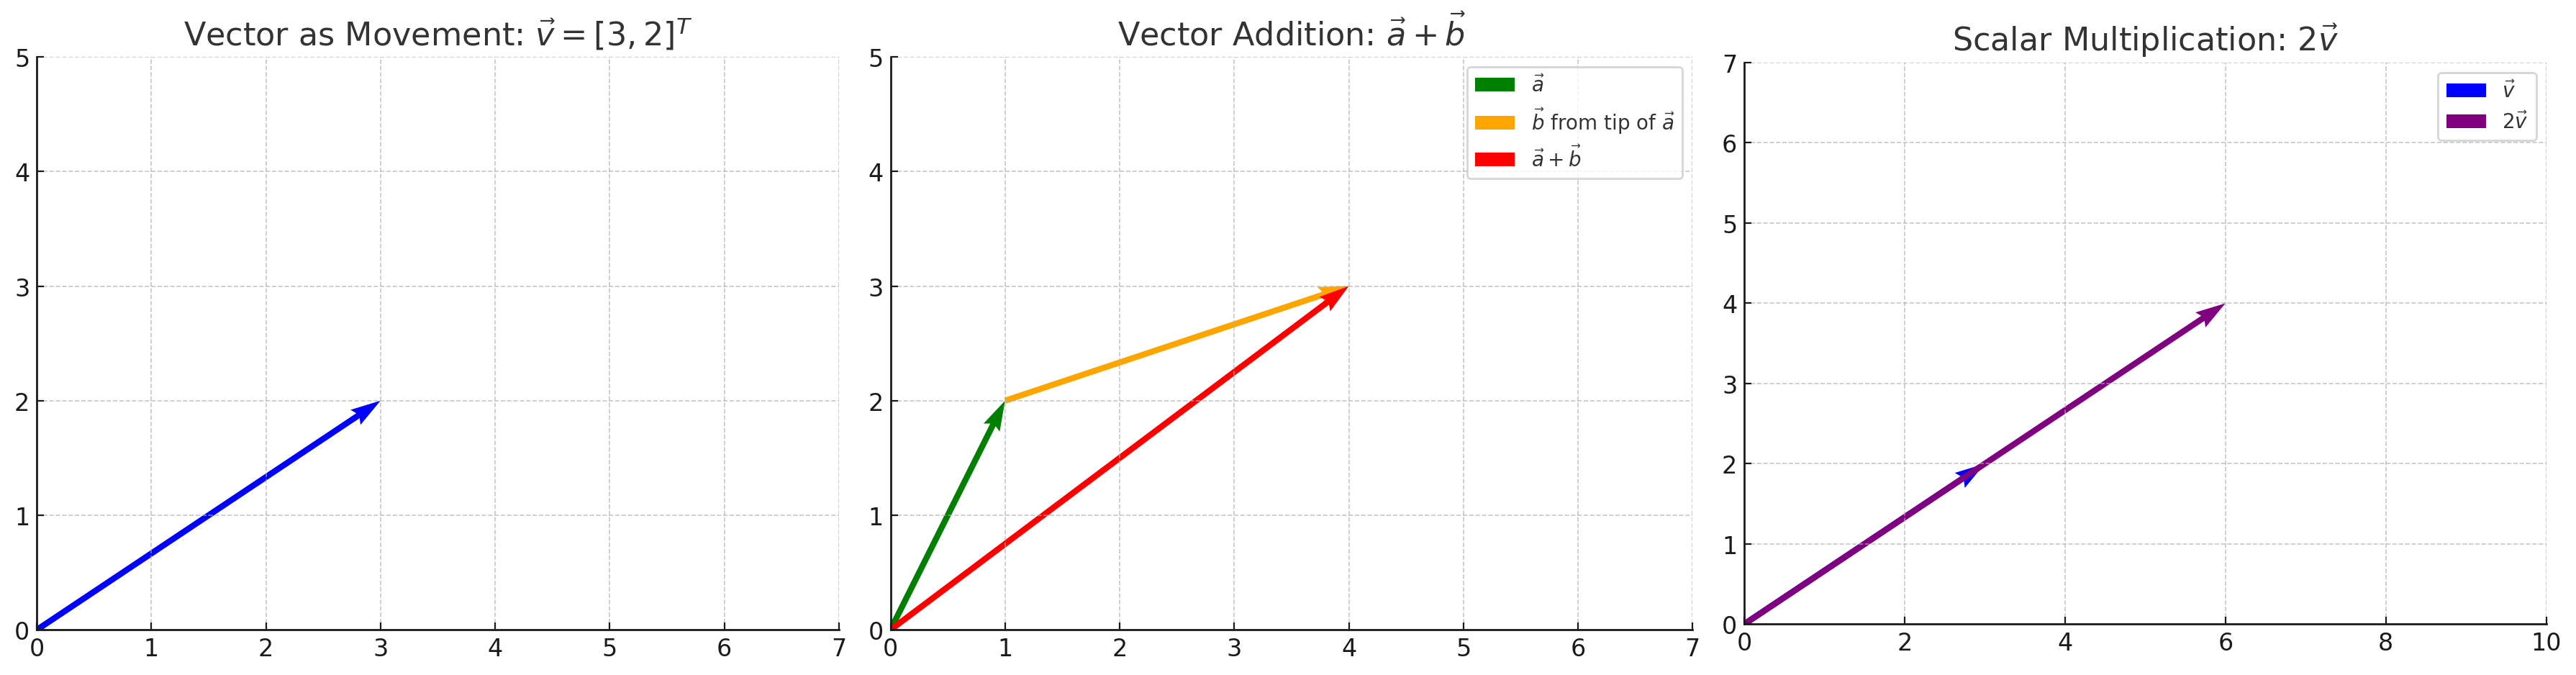
\includegraphics[width=\textwidth]{figures/vector_addition_multiplication.png}
	\caption{Visualizing vector movement, addition, and scalar multiplication.}
	\label{fig:vector_basics}
\end{figure}

Understanding vectors as movements in space lays the geometric foundation for understanding how they can be transformed, reshaped, and reoriented using linear transformations.

\section{The Philosophical Necessity of Linear Transformation in Image Processing}

To perceive is to transform. The world does not offer itself in neatly labeled form—it presents patterns, textures, and arrangements. To recognize structure within raw data, a system must transform it. In deep learning, particularly in image processing, this transformation begins with a fundamental operation: the \textit{linear transformation}.

An image, at its core, is a grid of intensity values—nothing more than an ordered collection of numbers. However, these values in their raw form do not convey structure or meaning. They must be reinterpreted. A linear transformation provides the means to do so.

\begin{definition}
	A linear transformation is a function \( T: \mathbb{R}^n \rightarrow \mathbb{R}^m \) that satisfies the following properties:
	\begin{align*}
		T(\mathbf{a} + \mathbf{b}) &= T(\mathbf{a}) + T(\mathbf{b}) \\
		T(c \cdot \mathbf{a}) &= c \cdot T(\mathbf{a})
	\end{align*}
\end{definition}

In other words, it respects the structure of the space—it preserves addition and scalar multiplication. Philosophically, this is vital: a linear transformation does not distort relationships arbitrarily; it reshapes space while maintaining consistency. It can stretch, rotate, reflect, or project—but it never bends.

In image processing, an image of dimension \( 28 \times 28 \) can be flattened into a vector in \( \mathbb{R}^{784} \). Passing this vector through a linear transformation reshapes it into a new space, potentially revealing latent patterns not apparent in the original pixel arrangement. This process is not simply numerical—it is perceptual. It reorients the data to make meaningful structures easier to extract.

\[
\mathbf{y} = A\mathbf{x}
\]

Here, \( \mathbf{x} \in \mathbb{R}^{n} \) is the input image vector, \( A \in \mathbb{R}^{m \times n} \) is the transformation matrix (learned in neural networks), and \( \mathbf{y} \in \mathbb{R}^m \) is the transformed representation.

\textit{Linear transformations do not merely shift numbers—they shift perspectives. They give a model the ability to perceive form within chaos.}



\section{Matrices Support Transformation}

\textit{At the heart of deep learning is the idea to learn from change.}  
This is not a poetic abstraction—it is a foundational truth. One of the many dimensions of Learning is the recognition that \textit{something is no longer the same as it was}. Whether in a biological mind or an artificial network, learning does not arise from repetition. For example, if a person is repeatedly making the same mistake then we can say that the person is not learning. Therefore, learning comes from \textit{difference}.

In the world of deep learning, we develop and train models that can make accurate predictions in the task that they have been developed and trained. During training stage, when a model makes an incorrect prediction, the misalignment between output and ground truth becomes the source of learning. It is not the prediction alone that teaches, nor the data alone—but the \textit{discrepancy} between the two. In other words, change is not an accident—it is the \textit{signal}. However, recognizing change is not enough. To learn from it, the system must represent it, measure it, and respond to it in a structured way. When we say a system must “represent” change, we are saying:
\begin{itemize}
	\item It must hold in memory some version of what has changed.
	\item It must structure that memory so that learning becomes possible.
\end{itemize}

So this representation must contain:
\begin{itemize}
	\item What is being changed (the values),
	\item How those values relate to others around them (the structure or pattern of change).
\end{itemize}

Learning doesn’t occur on values alone—it occurs on patterns in how those values interact. Imagine two examples:
\begin{itemize}
	\item If one pixel in an image becomes brighter, that’s a \textit{local} change.
	\item But if the whole region changes from “a cat” to “a dog,” that’s a \textit{structural} or \textit{relational} change.
\end{itemize}
To understand that, the model must not just know \textit{what} changed (value), but also:
\begin{itemize}
	\item Where it changed
	\item In relation to what
	\item How far that change propagates
\end{itemize}
So relationships matter: they tell us how changes in one place affect meaning in context and a Matrix help us Encode this.  

A matrix is a grid of numbers. But critically:
\begin{itemize}
	\item Each number (value) sits in a position (row, column).
	\item This position gives context: it tells us which values are near, which are far, and what kind of structure exists.
\end{itemize}

\textbf{Example:}
\[
\begin{bmatrix}
	5 & 5 & 5 \\
	5 & 10 & 5 \\
	5 & 5 & 5 \\
\end{bmatrix}
\]
Here, “10” is a value, but it's only meaningful because it’s surrounded by 5s.  
The matrix lets us perceive that the center stands out—this is a relational insight. So the matrix doesn't just store the value “10”, but also the fact that “10 is central, different, and structurally significant.” This structured way requires a data format that:
\begin{itemize}
	\item Stores values (what changed)
	\item Preserves relationships (how values relate across space or time)
\end{itemize}
This demands a form that can express both \textit{values and relationships}, a format that preserves the \textit{geometry of information}. That form is the \textbf{matrix}.Matrix doesn’t just hold numbers; it holds them \textit{in relation to one another}, giving us:
\begin{itemize}
	\item Local patterns
	\item Global structure
	\item The ability to transform both using algebra
\end{itemize}
Without matrices, the model would only have isolated data. With matrices, it can reason about form, flow, and pattern. A matrix is more than a table of numbers. It is a space in which \textit{relationships are embedded directly into structure}—where each element is not isolated but defined partly by its position. In image data, for instance, nearby pixels often carry related meaning; a matrix preserves this locality. In networks, weight matrices store learned transformations that map inputs to outputs—not just pointwise, but as \textit{global patterns of change}.

Moreover, the very act of learning—mathematically speaking—is guided by gradients, which are formal expressions of \textit{how a change in one value affects change in another}. These gradients are computed using \textit{matrix calculus}, and applied as updates to other matrices—weights, activations, filters. In this sense, matrices are not merely passive containers; they are the \textit{medium through which change flows and accumulates}.
\begin{quote}
	Learning from change requires more than memory. It requires a form that supports structured transformation. The matrix is that form—it both holds and evolves information, enabling the system to encode not only what \textit{is}, but how what \textit{is} can become something more.
\end{quote}

\section{Controlled Transformations}

\textit{To learn is not merely to observe change—it is to shape it.}  
A machine learning system does not passively witness variation; it seeks to modify its internal state in response to that variation, aiming to reduce error, increase accuracy, and discover structure. But such modification must be \textit{disciplined}, not random. Learning is effective only when the transformations it performs are \textbf{controlled}—that is, intentional, measurable, and adjustable.

In deep learning, transformation refers to the process by which one representation is mapped into another. This mapping is typically achieved through \textit{matrix multiplication}, where an input (such as a vector or a matrix) is multiplied by a weight matrix to produce a new form. But unlike traditional systems with fixed rules, deep learning models \textit{learn} the parameters of these transformations. The model does not begin with knowledge of how inputs should be transformed—it discovers those transformations over time, guided by a signal: the \textbf{gradient}.

The gradient provides the essential mechanism of control. It measures how small changes in each parameter affect the final error. Using this information, the model adjusts its transformation matrices to move toward lower error. This process—\textit{gradient descent}—is repeated iteratively, causing the system to slowly refine the structure of its transformations. In this sense, the matrix is not a static operator; it is a \textit{learnable transformation function}, evolving with experience.

This notion of control is crucial. If transformations were random or fixed, the system could not adapt to new data or improve from failure. What makes learning possible is the fact that transformation is \textit{both structured and malleable}. The matrix gives us the structure; the gradient gives us the malleability.

\begin{quote}
	In this view, learning becomes the art of discovering how to transform one state of representation into another—not by chance, but by adjusting internal transformations under the discipline of feedback. The matrix is the medium. The gradient is the guide. And the transformation is the soul of learning.
\end{quote}

\section{The Philosophy of Composition}

\textit{Complex understanding begins with simple parts.}  
This principle is not exclusive to deep learning; it is a general law of cognition, perception, and language. Our minds are structured to interpret the world not as a chaos of unrelated facts, but as \textit{systems of nested relationships}—layers of meaning that emerge from simpler building blocks.

In language, individual sounds form syllables, which become words. Words combine into phrases, and phrases into arguments. In vision, pixels form edges, edges form shapes, and shapes form objects. This compositional logic is not superficial—it is foundational. We do not merely observe the world; we build its meaning piece by piece.

Deep learning mirrors this process through architecture. A neural network does not attempt to leap from raw data to abstract conclusions in a single step. Instead, it applies a sequence of transformations—each layer refining, amplifying, or reorganizing what came before. These layers do not operate in isolation; they are \textit{composed}, meaning each one \textit{receives, modifies, and passes on} the work of the previous.

What emerges is a \textbf{hierarchy of representation}. The lower layers capture fine detail and local structure. Middle layers begin to recognize combinations and patterns. Higher layers abstract away from the specifics to form conceptual categories. But this ascent in abstraction is only possible because of \textbf{composition}—the deliberate layering of small, learnable transformations into a coherent whole.

\begin{quote}
	Composition is the scaffold of meaning. Without it, learning would remain flat and disconnected. With it, the system gains depth—not just in architecture, but in insight.
\end{quote}

\subsection{Why Convolutional Kernels Have Shape}

It is only in the context of neighboring pixels, and within the interpretive framework of a model or a mind, that any individual pixel becomes meaningful—whether as part of an edge, a shadow, or an object. A single pixel by itself does not represent structure; it must be situated within a surrounding region that reveals contrast, orientation, or spatial configuration.

This is precisely why convolutional kernels are designed with specific height and width.  
The kernel defines the \textit{local region of context} that the model will use to interpret the presence or absence of a pattern. By sliding this kernel across the image, the model is essentially asking, repeatedly:
\begin{quote}
	“Does this arrangement of pixels match a structure I’ve learned to recognize?”
\end{quote}

The choice of kernel size is not arbitrary—it encodes an assumption about \textit{how much context is necessary} to extract meaningful relationships. A $3 \times 3$ kernel captures very local structures, such as edges or corners. A $5 \times 5$ or larger kernel can capture more extended features—such as curves, textures, or small motifs. If the kernel is too small, it may miss global coherence; if too large, it may dilute local detail.

In this sense, the kernel is a kind of \textbf{window of perception}: it frames the portion of the visual field that the model is allowed to consider at once. The size of this window determines the \textit{scale of patterns} the model is capable of detecting. A kernel is therefore both a computational tool and a philosophical commitment—it defines what constitutes a “pattern” in the world, and how far the model must look to find one.


\section{Images as Structured Tensors}

In the context of deep learning, an image is not merely a visual representation but a structured numerical object—a tensor with defined dimensions and meaning. Mathematically, an image is represented as a three-dimensional tensor \( \mathbb{R}^{C \times H \times W} \), where \( C \) denotes the number of color channels (e.g., 3 for RGB), and \( H \) and \( W \) refer to the image’s height and width in pixels. When processed in batches during training, this tensor extends to four dimensions \( \mathbb{R}^{N \times C \times H \times W} \), with \( N \) representing the batch size. This format is standard in frameworks like PyTorch, while TensorFlow typically adopts the \( N \times H \times W \times C \) layout. 

Despite their numerical structure, these pixel values—intensities normalized between 0 and 1 or rescaled—carry no inherent semantic content. A value such as 182, for instance, is just a scalar unless it is interpreted within a channel and spatial configuration. The convolutional layer receives this tensor and treats it as a raw signal. It is not the pixel values in isolation but rather their arrangement and proximity that lay the groundwork for meaningful interpretation. Thus, even before learning begins, the architecture presumes that information is spatially organized, and that meaning—if any—is embedded in relationships, not in individual values.

\begin{lstlisting}[caption=Creating and passing an image through a Conv2d layer in PyTorch]
	import torch
	
	# A batch of 1 image, with 3 channels, 32x32 pixels
	image = torch.randn(1, 3, 32, 32)
	
	import torch.nn as nn
	conv = nn.Conv2d(in_channels=3, out_channels=16, kernel_size=3, padding=1)
	output = conv(image)
\end{lstlisting}

\begin{lstlisting}[caption=Creating and passing an image through a Conv2D layer in TensorFlow]
	import tensorflow as tf
	
	# A batch of 1 image, shape: (batch_size, height, width, channels)
	image = tf.random.normal([1, 32, 32, 3])
	
	conv = tf.keras.layers.Conv2D(filters=16, kernel_size=3, padding='same')
	output = conv(image)
\end{lstlisting}


\section{Contextualizing Semantic Meaning}

The notion of "meaning" in data processing, particularly in deep learning, requires careful qualification. A single numerical value—such as a pixel intensity—does not possess semantic significance on its own. To understand this more precisely, it is helpful to distinguish between structural, syntactic, and semantic meaning. \textbf{Structural information} refers to how elements are arranged—for example, the shape of a matrix or the order of words in a sentence. In an image, this could correspond to the layout of pixel rows and columns. \textbf{Syntactic information}, in turn, involves formal rules that govern how elements can be combined. For instance, in programming, syntax dictates how variables and operations can be combined legally; in language, it tells us that a sentence must have a subject and a verb. These structural and syntactic patterns define form, but not content.

\paragraph{Example of Structural Information.}
In natural language, structural information refers to the order of words. For instance, the two sentences:
\begin{quote}
	\textit{``The cat chased the mouse.''} \\
	\textit{``The mouse chased the cat.''}
\end{quote}
contain the same words and obey grammatical rules, but their structure leads to entirely different interpretations due to the changed positions of subject and object.

In image data, structure corresponds to the spatial arrangement of pixels. For example, a 3$\times$3 matrix of pixel values like:
\[
\begin{bmatrix}
	100 & 100 & 100 \\
	0 & 0 & 0 \\
	100 & 100 & 100 \\
\end{bmatrix}
\]
may suggest a horizontal edge due to the contrast between rows, a pattern that would not exist if the same values were shuffled randomly.

\paragraph{Example of Syntactic Information.}
In programming languages, syntax dictates how symbols must be arranged. The expression:
\begin{quote}
	\texttt{int x = 5;}
\end{quote}
is syntactically correct in C++, whereas:
\begin{quote}
	\texttt{int = x 5;}
\end{quote}
is not, even though it uses the same tokens. The syntax defines which forms are valid, not what the variables or values represent.

In deep learning, syntactic rules may refer to tensor compatibility. For example, attempting to multiply a tensor of shape $(3 \times 4)$ with a tensor of shape $(5 \times 6)$ will result in an error, not because of semantic issues, but because the operation is syntactically invalid under matrix multiplication rules.


\textbf{Semantic meaning}, on the other hand, pertains to what something \emph{refers to} or \emph{implies} in a given context. In natural language, the word “bank” has different semantic interpretations depending on context—it may refer to a financial institution or the edge of a river. Similarly, in an image, a pixel value of 182 in the red channel is just a number unless it is part of a spatial pattern that may represent, for instance, the curvature of a handwritten digit or the contour of a car. In convolutional networks, it is not the absolute values of pixels that carry semantic weight but their patterns of co-occurrence across space and channels. These relationships make it possible for a model to infer edges, textures, and object parts—not because any single pixel is meaningful, but because groups of pixels form structures that align with higher-level concepts. Hence, semantics are not properties of isolated numbers but emerge through structured, relational interpretation.

\section{The Role of the Convolutional Layer}

A convolutional layer is a fundamental building block in deep learning models for processing spatially structured data such as images. It operates by sliding a set of small filters, or kernels, over the input tensor to produce feature maps that capture local patterns. Each filter performs a dot product between its weights and a local patch of the input, effectively highlighting specific types of local variation. However, at initialization, these filters are randomly assigned and have no prior knowledge of what constitutes a meaningful feature. The convolution operation itself encodes only a structural prior: the assumption that useful information is often localized and translationally invariant. It provides a mechanism for detecting patterns, but not for determining which patterns are significant.

The filters gain semantic relevance only through training. As data is passed through the network and predictions are compared to known targets, feedback in the form of gradients adjusts the weights of the filters. Over time, this process causes the filters to specialize in detecting features that are useful for the task—such as edges, textures, and object parts. The key insight here is that convolutional layers do not explicitly extract semantic features because they have been told what to look for; rather, they extract features that emerge as semantically meaningful because they help reduce the model’s error. Thus, the role of the convolutional layer is not to encode meaning directly, but to provide a structured interface through which meaningful patterns can be discovered via optimization.

\begin{lstlisting}[caption=Training a convolutional layer: random initialization and learning via gradient descent]
	import torch
	import torch.nn as nn
	import torch.optim as optim
	
	# Define a simple Conv2D layer followed by flattening and linear output
	conv = nn.Conv2d(in_channels=3, out_channels=2, kernel_size=3, padding=1)
	linear = nn.Linear(2 * 32 * 32, 10)  # e.g., 10-class classification
	
	# Combine into a simple model
	model = nn.Sequential(conv, nn.Flatten(), linear)
	
	# Dummy image and label
	image = torch.randn(1, 3, 32, 32)         # input image
	target = torch.randint(0, 10, (1,))       # random class label
	
	# Define loss and optimizer
	criterion = nn.CrossEntropyLoss()
	optimizer = optim.SGD(model.parameters(), lr=0.01)
	
	# Forward pass
	output = model(image)
	loss = criterion(output, target)
	
	# Backward pass and update
	optimizer.zero_grad()
	loss.backward()
	optimizer.step()
\end{lstlisting}

\section{Emergence of Semantics Through Optimization}

The ability of neural networks to extract semantically meaningful features does not arise from the mechanics of convolution or gradient descent alone. Gradient descent is a purely numerical procedure; it does not encode domain knowledge or interpretative goals. Its function is to iteratively minimize a loss function by adjusting the model's weights in response to observed errors. As such, it responds only to whether a prediction is closer to or further from a desired target. The semantic orientation of the features—such as whether a learned filter detects an eye, an edge, or a tail—is not embedded in the algorithm, but is a consequence of the \emph{structure} of the task. Specifically, the loss function, paired with labeled data, defines what counts as success. This definition then drives the network to prioritize features that improve performance on that task.

As training progresses, features that consistently help reduce loss are reinforced, while uninformative features are suppressed. In this way, filters gradually specialize—not due to an explicit semantic signal, but because semantic features tend to be functionally useful in minimizing task-specific error. For example, in a dog-vs-cat classifier, filters that respond to fur texture, ear shape, or eye placement become statistically favorable because they help differentiate between the two classes. These features \emph{acquire} semantic meaning as a side effect of being useful. Therefore, the emergence of semantics is not the result of direct supervision on meaning itself, but rather of a system that, through task performance, converges on patterns that align with meaningful structure in the data.

\begin{lstlisting}[caption=Semantics emerge from loss-driven adaptation rather than explicit supervision]
	import torch
	import torch.nn as nn
	import torch.optim as optim
	
	# A small CNN for binary classification (e.g., cat vs dog)
	class SmallCNN(nn.Module):
	def __init__(self):
	super().__init__()
	self.conv = nn.Conv2d(3, 8, 3, padding=1)  # 8 random filters
	self.pool = nn.AdaptiveAvgPool2d((1, 1))
	self.fc = nn.Linear(8, 2)  # Binary classifier
	
	def forward(self, x):
	x = torch.relu(self.conv(x))  # Learn features via ReLU
	x = self.pool(x).view(x.size(0), -1)
	return self.fc(x)
	
	model = SmallCNN()
	optimizer = optim.Adam(model.parameters(), lr=0.001)
	criterion = nn.CrossEntropyLoss()
	
	# Training step (simulated)
	image = torch.randn(1, 3, 64, 64)               # Input image
	label = torch.tensor([1])                      # Target class: e.g., "dog"
	
	# Forward, backward, update
	output = model(image)
	loss = criterion(output, label)
	optimizer.zero_grad()
	loss.backward()
	optimizer.step()
\end{lstlisting}




\chapter{Common Python Code}
\section{Python Data Types and Cheat Sheet}

This section summarizes essential Python and PyTorch data structures and functions, with an emphasis on their abstract categories (e.g., \textit{mapping}, \textit{sequence}, \textit{iterable}). Understanding these abstractions is critical for reasoning about how different operations behave, what inputs they expect, and what types they return.

\subsection*{1. Fundamental Data Structures and Concepts}

\begin{description}
	\item[\textbf{list}] An \textbf{ordered}, \textbf{mutable} sequence of elements, indexed by position. Supports operations like indexing, slicing, and mutation.
	\begin{lstlisting}[language=Python]
		words = ["hello", "world"]
		words[0]  # "hello"
		words.append("!")
	\end{lstlisting}
	
	\item[\textbf{dict}] A \textbf{mapping} from unique keys to values. Provides fast lookup and update using \texttt{key} syntax.
	\begin{lstlisting}[language=Python]
		word2idx = {"cat": 0, "dog": 1}
		word2idx["cat"]  # 0
	\end{lstlisting}
	
	\item[\textbf{Mapping}] An abstract interface for any object that supports key-value access. Includes \texttt{dict}, \texttt{Counter}, etc. Formally: $f : K \rightarrow V$.
	
	\item[\textbf{Iterable}] Any object usable in a \texttt{for} loop or comprehension. Includes lists, strings, sets, dicts, and ranges.
	
	\item[\textbf{Sequence}] A special kind of iterable that is \textbf{ordered} and \textbf{indexable}. Includes \texttt{list}, \texttt{tuple}, \texttt{str}, \texttt{range}.
	
	\item[\textbf{Counter}] A \texttt{dict}-like object from \texttt{collections} that counts element frequency in an iterable.
	\begin{lstlisting}[language=Python]
		from collections import Counter
		Counter(["apple", "apple", "banana"])  # {'apple': 2, 'banana': 1}
	\end{lstlisting}
	
	\item[\textbf{torch.Tensor}] A multi-dimensional numeric array (vector, matrix, etc.) used in PyTorch. Efficiently supports math and GPU acceleration.
	\begin{lstlisting}[language=Python]
		import torch
		x = torch.tensor([1.0, 2.0, 3.0])
		x.size()  # torch.Size([3])
	\end{lstlisting}
\end{description}

\subsection*{2. Python \& PyTorch Cheat Sheet (with Types)}

\begin{table}[h!]
	\centering
	\renewcommand{\arraystretch}{1.3}
	\begin{tabular}{|>{\ttfamily}l|l|l|l|}
		\hline
		\textbf{Function} & \textbf{Purpose} & \textbf{Input Type} & \textbf{Output Type} \\
		\hline
		text.lower() & Lowercase conversion & str & str \\
		text.replace() & Replace substring & str, str, str & str \\
		re.sub() & Regex substitution & str, str, str & str \\
		text.split() & Split string by space & str & List[str] \\
		\hline
		Counter(iterable) & Frequency counter & Iterable[Any] & Counter (dict-like) \\
		counter.update() & Add counts & Iterable[Any] & None \\
		counter.items() & Key-value pairs & Counter & Iterable[Tuple[Any, int]] \\
		\hline
		Dict[key] & Direct key lookup & Mapping, key & value \\
		Dict.get(k, d) & Key lookup with default & Mapping, key, default & value \\
		len(Dict) & Size of mapping & Mapping & int \\
		\hline
		{[}f(x) for x in it] & List comprehension & Iterable & List \\
		\{k: v for ...\} & Dict comprehension & Iterable & Dict \\
		\hline
		lst.append(x) & Append item & List, item & None (mutates) \\
		lst + [x] & Create new list & List & List \\
		lst.extend(it) & Add multiple items & List, Iterable & None (mutates) \\
		\hline
		torch.tensor(data) & Create tensor & Sequence, array & Tensor \\
		tensor.size() & Shape of tensor & Tensor & torch.Size \\
		\hline
	\end{tabular}
	\caption{Python and PyTorch function cheat sheet with input and output types}
\end{table}

\subsection*{3. Conceptual Categories Summary}

\begin{table}[h!]
	\centering
	\renewcommand{\arraystretch}{1.3}
	\begin{tabular}{|l|l|l|}
		\hline
		\textbf{Class or Type} & \textbf{Category} & \textbf{Core Properties} \\
		\hline
		\texttt{list} & Sequence & Ordered, mutable, indexed \\
		\texttt{dict} & Mapping & Key-value pairs, fast lookup \\
		\texttt{Counter} & Mapping subclass & Frequency count, iterable keys \\
		\texttt{Iterable} & Abstract type & For loops, comprehensions \\
		\texttt{Sequence} & Indexed iterable & Supports slicing/indexing \\
		\texttt{Mapping} & Abstract type & Provides key $\rightarrow$ value access \\
		\texttt{torch.Tensor} & Numeric container & Multi-dimensional, mathematical \\
		\hline
	\end{tabular}
	\caption{Summary of common Python object categories}
\end{table}

\section{Typical Function Categories in Python Programming}

Understanding functions in terms of their high-level behavior rather than only their syntax is essential for reasoning, abstraction, and clean program design. This section outlines typical categories of functions and operations used in Python, particularly in the context of data processing, machine learning, and model pipelines.

\subsection*{1. Transformation Functions}

These functions take an input (often a sequence, string, or tensor) and return a modified version — usually with the same type but altered content.

\begin{itemize}
	\item \textbf{Purpose:} To convert, modify, or reformat data.
	\item \textbf{Does not mutate} the original input (usually).
\end{itemize}

\textbf{Examples:}

\begin{itemize}
	\item \texttt{text.lower()} – Converts text to lowercase (\texttt{str} $\rightarrow$ \texttt{str})
	\item \texttt{sorted(lst)} – Returns a sorted copy of a list
	\item \texttt{re.sub(...)} – Returns a string with regex-based substitutions
	\item \texttt{torch.tensor([...])} – Converts list to tensor
\end{itemize}

\subsection*{2. Aggregation Functions}

These reduce a collection (list, iterable, or tensor) to a single value or statistic.

\begin{itemize}
	\item \textbf{Purpose:} Summarize or compress data into scalar form.
	\item \textbf{Typically returns:} \texttt{int}, \texttt{float}, or small tuple.
\end{itemize}

\textbf{Examples:}

\begin{itemize}
	\item \texttt{len(lst)} – Number of elements
	\item \texttt{sum(numbers)} – Sum of a list or iterable
	\item \texttt{max(values)} – Maximum value
	\item \texttt{tensor.mean()} – Mean of tensor values
\end{itemize}

\subsection*{3. Mutation Functions}

These directly change (mutate) the object they operate on. They are typically used with mutable data structures like lists or dictionaries.

\begin{itemize}
	\item \textbf{Purpose:} Change the input object in place.
	\item \textbf{Typically returns:} \texttt{None}, but changes the object.
\end{itemize}

\textbf{Examples:}

\begin{itemize}
	\item \texttt{lst.append(x)} – Adds element to list
	\item \texttt{lst.extend(other)} – Concatenates another list
	\item \texttt{dict.update(...)} – Adds or updates keys
	\item \texttt{counter.update(tokens)} – Increments internal counts
\end{itemize}

\subsection*{4. Accessor Functions}

These retrieve information from a data structure without modifying it. They may expose structure, shape, or metadata.

\begin{itemize}
	\item \textbf{Purpose:} Inspect or extract properties from data.
\end{itemize}

\textbf{Examples:}

\begin{itemize}
	\item \texttt{dict[key]} – Access value by key
	\item \texttt{word2idx.get(key, default)} – Safe key lookup
	\item \texttt{tensor.size()} – Returns shape of a tensor
	\item \texttt{counter.items()} – Returns key-count pairs
\end{itemize}

\subsection*{5. Generator Expressions and Comprehensions}

These build new data structures (lists, dicts, sets) from iterables using inline expressions.

\begin{itemize}
	\item \textbf{Purpose:} Compactly construct a transformed collection.
	\item \textbf{Type returned:} \texttt{list}, \texttt{dict}, \texttt{set}, or generator.
\end{itemize}

\textbf{Examples:}

\begin{itemize}
	\item \texttt{[x**2 for x in nums]} – Square all elements
	\item \texttt{\{k: v for k, v in zip(K, V)\}} – Build dict from key-value pairs
	\item \texttt{(x for x in lst)} – Lazy generator expression
\end{itemize}

\subsection*{6. Conversion or Casting Functions}

These convert objects from one type to another.

\begin{itemize}
	\item \textbf{Purpose:} Enforce type expectations or adapt structure.
\end{itemize}

\textbf{Examples:}

\begin{itemize}
	\item \texttt{list(...)} – Convert iterable to list
	\item \texttt{dict(...)} – Convert key-value iterable to dict
	\item \texttt{torch.tensor(...)} – Convert list/array to tensor
	\item \texttt{str(number)} – Convert number to string
\end{itemize}

\subsection*{Summary Table: Function Categories}

\begin{table}[h!]
	\centering
	\renewcommand{\arraystretch}{1.3}
	\begin{tabular}{|l|l|l|}
		\hline
		\textbf{Category} & \textbf{Purpose} & \textbf{Typical Output Type} \\
		\hline
		Transformation & Modify or reshape input & Same or similar to input type \\
		Aggregation & Summarize input & Scalar or tuple \\
		Mutation & Modify input object in-place & Usually None \\
		Accessor & Retrieve value or property & Any \\
		Comprehension & Construct new iterable structure & list, dict, set, generator \\
		Conversion & Change type or format & Target type (e.g., str, list, tensor) \\
		\hline
	\end{tabular}
	\caption{Conceptual classification of Python functions}
\end{table}

\section{The Pattern of Sequence Padding and Length Normalization}

In many computational tasks, particularly in deep learning and signal processing, it is necessary to normalize the length of input sequences. This normalization ensures that downstream models, which typically require fixed-size input, can process data uniformly in batches.

A common and efficient strategy for length normalization is the \textbf{sequence padding pattern}, often implemented using list multiplication and in-place augmentation.

\subsection*{Motivation}

\begin{itemize}
	\item Neural networks (e.g., RNNs, Transformers) expect inputs of the same length within a batch.
	\item Algorithms such as dynamic programming rely on consistent dimensionality.
	\item Hardware accelerators like GPUs and TPUs are optimized for fixed-size tensor operations.
\end{itemize}

To accommodate variable-length sequences, we use padding as a uniformity mechanism.

\subsection*{General Pattern}

The typical logic for padding a sequence to a desired length is:

\begin{lstlisting}[language=Python, caption={Basic sequence padding pattern}]
	if len(sequence) < desired_length:
	padding = [pad_value] * (desired_length - len(sequence))
	sequence += padding
\end{lstlisting}

\subsection*{Constituent Components}

\begin{table}[h]
	\centering
	\begin{tabular}{|p{3cm}|p{3cm}|p{7cm}|}
		\hline
		\textbf{Component} & \textbf{Role} & \textbf{Explanation} \\
		\hline
		\texttt{sequence} & Variable-length input & A list or tensor representing text, time series, or signal \\
		\texttt{desired\_length} & Target fixed length & Required for batching or downstream model constraints \\
		\texttt{pad\_value} & Padding element & Neutral value used to fill extra positions (e.g., 0 or \texttt{"<PAD>"}) \\
		\texttt{len(sequence)} & Length check & Determines how much padding is needed \\
		\texttt{[pad\_value] * n} & List multiplication & Efficiently creates repeated padding values \\
		\texttt{+=} & In-place update & Extends the sequence without copying \\
		\hline
	\end{tabular}
	\caption{Constituents of the sequence padding pattern}
\end{table}

\subsection*{Applications}

\begin{itemize}
	\item \textbf{Natural Language Processing:} Padding tokenized text to a fixed length for model input.
	\item \textbf{Audio/Signal Processing:} Padding audio frames to fixed window sizes.
	\item \textbf{Computer Vision:} Padding cropped regions or object masks for convolution.
	\item \textbf{Time Series Forecasting:} Padding sequences to align time steps across samples.
	\item \textbf{Dynamic Programming:} Initializing DP tables with base values.
\end{itemize}

\subsection*{Truncation: The Inverse Operation}

If the sequence is longer than required, truncation is applied:

\begin{lstlisting}[language=Python, caption={Truncating a sequence to desired length}]
	if len(sequence) > desired_length:
	sequence = sequence[:desired_length]
\end{lstlisting}

This is useful when only the initial segment is needed, especially in memory-constrained settings.

\subsection*{Summary}

The padding pattern is a reusable preprocessing strategy for converting variable-length inputs into fixed-length representations. It plays a foundational role in enabling batch computation and efficient model training. Its components are simple yet powerful, and it generalizes across a wide range of domains including NLP, vision, and time-series modeling.

\section{Building Token Frequencies with \texttt{collections.Counter}}

\paragraph{Motivation.}
When processing text data, we often want to know how many times each word appears across a corpus. This frequency information is essential for building vocabularies, filtering rare words, or weighting features. Python’s \texttt{collections.Counter} provides a simple and efficient way to do this.

\subsection{What is \texttt{Counter}?}

\texttt{Counter} is a dictionary subclass from Python's \texttt{collections} module that is specifically designed to count hashable objects.

\begin{lstlisting}[language=Python, caption={Basic Counter example}]
	from collections import Counter
	
	words = ["apple", "banana", "apple", "orange", "banana", "apple"]
	counter = Counter(words)
	
	print(counter)
\end{lstlisting}

\textbf{Output:}
\begin{lstlisting}[language=Python]
	Counter({'apple': 3, 'banana': 2, 'orange': 1})
\end{lstlisting}

\paragraph{Explanation.}
Each unique element in the list is counted, and the result is stored as a dictionary-like object. The keys are the elements, and the values are the counts.

\subsection{Using \texttt{Counter.update()}}

You can also use \texttt{counter.update()} to add counts incrementally from another iterable.

\begin{lstlisting}[language=Python, caption={Updating a Counter with more data}]
	counter = Counter()
	counter.update(["apple", "banana"])
	counter.update(["apple", "orange"])
	
	print(counter)
\end{lstlisting}

\textbf{Output:}
\begin{lstlisting}[language=Python]
	Counter({'apple': 2, 'banana': 1, 'orange': 1})
\end{lstlisting}

\paragraph{Explanation.}
The update function takes an iterable (like a list of words) and adds the counts of each element to the existing values in the counter.

\subsection{Applying to Tokenized Text Data}

In NLP, we often have a list of tokenized sentences — each sentence is a list of words. Our goal is to count how often each word appears in the full dataset.

\begin{lstlisting}[language=Python, caption={Counting word frequencies across multiple sentences}]
	tokenized_sentences = [
	["i", "love", "this", "movie"],
	["i", "do", "not", "love", "this", "movie"]
	]
	
	counter = Counter()
	for tokens in tokenized_sentences:
	counter.update(tokens)
	
	print(counter)
\end{lstlisting}

\textbf{Output:}
\begin{lstlisting}[language=Python]
	Counter({'i': 2, 'love': 2, 'this': 2, 'movie': 2, 'do': 1, 'not': 1})
\end{lstlisting}

\paragraph{Explanation.}
We initialize an empty counter and iterate through each list of tokens (i.e., each sentence). At each step, \texttt{update(tokens)} adds the count of every word in that sentence to the cumulative counter.

\begin{itemize}
	\item The token ``i'' appears in both sentences → count is 2.
	\item ``love'', ``this'', and ``movie'' also appear twice.
	\item ``do'' and ``not'' only appear in the second sentence → count is 1.
\end{itemize}

This is the standard method for computing word frequencies when building vocabularies from tokenized corpora.

\section{Understanding \texttt{torch.zeros()} in PyTorch}

The function \texttt{torch.zeros()} is a core tensor constructor in PyTorch that creates a tensor filled entirely with zeros. It is especially useful for initializing variables, defining placeholder tensors, or creating empty input templates.

\subsection{Function Signature}
\begin{itemize}
	\item \texttt{torch.zeros(size, dtype=None, device=None, requires\_grad=False)}
\end{itemize}

\begin{itemize}
	\item \textbf{\texttt{size}}: A tuple or list specifying the shape of the output tensor.
	\item \textbf{\texttt{dtype}} (optional): The desired data type (e.g., \texttt{torch.float}, \texttt{torch.int}).
	\item \textbf{\texttt{device}} (optional): The device on which to allocate the tensor, such as \texttt{'cpu'} or \texttt{'cuda'}.
	\item \textbf{\texttt{requires\_grad}} (optional): If set to \texttt{True}, operations on the tensor will be tracked for automatic differentiation.
\end{itemize}

Let us see how to create a 1D Tensor of Zeros

\begin{lstlisting}[language=Python, caption={Create a 1D tensor with 5 zeros}]
	import torch
	x = torch.zeros(5)
	print(x)
	# Output: tensor([0., 0., 0., 0., 0.])
\end{lstlisting}

Let us see  how to create a 2D Tensor of Zeros

\begin{lstlisting}[language=Python, caption={Create a 2D tensor with shape (3, 4)}]
	x = torch.zeros(3, 4)
\end{lstlisting}

Let us see how to specify Data Type and Device

\begin{lstlisting}[language=Python, caption={Using dtype and device parameters}]
	x = torch.zeros(2, 2, dtype=torch.int32, device='cpu')
\end{lstlisting}

Let us see how to enable Gradient Tracking

\begin{lstlisting}[language=Python, caption={Tensor that supports autograd}]
	x = torch.zeros(2, 2, requires_grad=True)
\end{lstlisting}

\paragraph{Common Use Cases}
\begin{itemize}
	\item Initializing model parameters such as weights and biases with zeros.
	\item Creating blank input templates or intermediate buffers.
	\item Padding inputs for sequence models or convolutional layers.
	\item Masking elements in attention mechanisms or loss computations.
\end{itemize}




\chapter{Spatially Local Pattern}
In deep learning, especially in image processing, \textbf{spatially local patterns} refer to features like edges, corners, and textures that appear within small regions of an image. This concept is fundamental to the study of how \textbf{Convolutional Neural Networks (CNNs)} learn to detect objects. CNNs use small filters (kernels) to scan across an image and detect local features that later combine into high-level concepts.
\chapter{Subtraction as a Fundamental Tool for Change Detection}
\section{Introduction}
Change detection lies at the core of numerous computational and cognitive tasks, spanning domains such as image processing, time-series forecasting, and symbolic reasoning. One of the most foundational yet powerful operations used to detect change is subtraction: the expression $A - B$. In this chapter, we present a logically structured argument for why subtraction serves as an effective and universal indicator of change. We investigate this idea from temporal, visual, and geometric perspectives, showing how this simple operation captures both magnitude and direction of change.
\section{Mathematical and Logical Basis of Subtraction}
Subtraction is defined as a binary operation that measures the difference between two quantities. Formally, given two scalars $A$ and $B$, the expression $A - B$ indicates the amount by which $A$ exceeds $B$, or the directional shift from $B$ to $A$. This operation inherently provides a three-way logical categorization:
\begin{itemize}
	\item $A - B > 0$: Positive change
	\item $A - B = 0$: No change
	\item $A - B < 0$: Negative change
\end{itemize}

This categorization underpins the logical use of subtraction in systems where change, deviation, or novelty must be identified. It transforms a passive comparison into an actionable, direction-sensitive insight.
\section{Subtraction in Temporal and Logical Structures}
In time-series data, systems are modeled as sequences of values indexed over time. The expression $x_t - x_{t-1}$ computes the change between successive time steps. This operation removes prior state information, isolating what is new. From a logical standpoint, subtraction here acts as a form of \emph{contrastive reasoning}: it eliminates what is already known (the past state) and retains only what has changed (the present deviation).

This idea extends to structured symbolic representations such as graphs or knowledge embeddings. In logical anomaly detection frameworks like ComAD or SINBAD, each relation or node is encoded as a vector. Subtracting an expected relationship $f(B)$ from an observed one $f(A)$ gives:
\[
\Delta = f(A) - f(B)
\]
This vector $\Delta$ captures the semantic deviation. The subtraction removes commonalities and reveals contradiction or novelty. Thus, logical reasoning is achieved through algebraic difference.
\section{Subtraction in Visual and Spatial Domains}
In image processing, edges—points of abrupt intensity change—can be detected using filters that apply subtraction across spatially neighboring pixels. A common example is the Sobel filter used for horizontal edge detection:
\[
K = \begin{bmatrix}
	-1 & 0 & 1 \\
	-2 & 0 & 2 \\
	-1 & 0 & 1 \\
\end{bmatrix}
\]
This kernel applies the expression $(\text{right intensity}) - (\text{left intensity})$, highlighting areas with strong horizontal contrast. The center row is weighted more because real images often carry more structural information in the center.

Here, subtraction works locally but serves a global purpose: it marks boundaries and discontinuities. The logic is again contrastive—only differences survive the operation.
\section{Geometric Reasoning and Directionality of Change}
In vector spaces, subtraction is geometrically interpreted as a directional vector from point $B$ to point $A$. That is:
\[
A - B = \vec{v} \Rightarrow \text{a vector pointing from } B \text{ to } A
\]

The direction of $\vec{v}$ reveals \emph{where} the change is occurring, and its magnitude $\|\vec{v}\|$ quantifies \emph{how much} change has occurred. This geometric reasoning is fundamental to modern machine learning systems, especially those relying on embedding spaces. For example, in word embeddings, the analogy:
\[
\text{king} - \text{man} + \text{woman} \approx \text{queen}
\]
works because subtraction captures the relational transformation: the difference between "king" and "man" is transferred to "woman".

Subtraction thus enables two forms of reasoning:
\begin{itemize}
	\item \textbf{Directional reasoning:} Determining how one state shifts toward another.
	\item \textbf{Contrastive reasoning:} Isolating what is different by removing what is shared.
\end{itemize}

This makes it a powerful tool in tasks requiring spatial reasoning, semantic change detection, and logical contradiction modeling.
\section{Subtraction in Natural Language Processing}
Subtraction has also emerged as a critical mechanism in Natural Language Processing (NLP), particularly in the context of word and sentence embeddings. Vector representations of words in models such as Word2Vec, GloVe, and BERT encode not only meaning but also relationships. For example, the well-known analogy:
\[
\text{king} - \text{man} + \text{woman} \approx \text{queen}
\]
relies on vector subtraction to isolate the concept of "royalty" and transfer it across gender. Here, subtraction is used to identify and preserve a relation while transforming other aspects of meaning.

Moreover, in tasks such as paraphrase detection, sentence similarity, or entailment, subtraction between sentence embeddings $f(A) - f(B)$ is used to measure dissimilarity. A small resulting vector indicates high semantic overlap, while a larger vector suggests differing meanings. This approach follows the same logical principle: remove what is shared and analyze what remains.

\subsection*{Where Does Semantic Meaning Come From?}
Semantic refers to \emph{meaning}—how concepts relate to one another. For example, the words \texttt{cat} and \texttt{dog} are semantically similar because they refer to animals of the same category. In contrast, \texttt{cat} and \texttt{car} are semantically unrelated despite some phonetic similarity.

An \emph{embedding} is a numeric vector that represents a word or sentence in a high-dimensional space. For instance:
\begin{itemize}
	\item \texttt{cat} $\rightarrow$ $[0.5, -1.2, 0.3, \dots]$
	\item \texttt{dog} $\rightarrow$ $[0.52, -1.15, 0.29, \dots]$
\end{itemize}
These vectors are close in space because the model has learned they are used in similar contexts.

Now consider the vectors for \texttt{king} and \texttt{man}. Subtraction gives:
\[
\texttt{king} - \texttt{man} = [0.5, 0.5, 0.3, \dots]
\]
This vector represents what makes a king different from a man—concepts like royalty or status.

When we add this difference to \texttt{woman}:
\[
\texttt{king} - \texttt{man} + \texttt{woman} \approx \texttt{queen}
\]
The model captures that "queen" is to "woman" what "king" is to "man." This kind of analogy only works because subtraction isolates semantic relationships.

Importantly, these relationships are learned by exposing the model to large corpora of language. If a model frequently sees "king rules kingdom" and "queen rules kingdom," it learns that both \texttt{king} and \texttt{queen} are related to rulership. It places them in a vector space where this pattern can be mathematically retrieved through subtraction.

In summary, subtraction in NLP works because embeddings store relational meaning. The vector $A - B$ captures "how $A$ differs from $B$ semantically," and when applied in analogy or similarity tasks, it provides a mechanism for detecting or transforming meaning.

\subsection*{Step-by-Step Semantic Reasoning with Embeddings}

\paragraph{1. What do we mean by \textquotedblleft semantic\textquotedblright?}
Semantic refers to \emph{meaning}—not spelling, not structure, but what a word or concept represents in context.

\textbf{Example:}
\begin{itemize}
	\item The words \texttt{apple} and \texttt{banana} are semantically close because both refer to fruits.
	\item The words \texttt{apple} and \texttt{laptop} may be semantically related only because of the company Apple, not in the food sense.
\end{itemize}
So when we say two words are semantically similar, we mean: \emph{“they appear in similar contexts or serve similar roles in language.”}

\paragraph{2. What is an embedding?}
An \emph{embedding} is a vector representation of a concept (word, sentence, etc.) that captures its semantic context in numerical form.

\textbf{Example:} In a model like Word2Vec:
\begin{align*}
	\texttt{cat} &= [0.5, -1.2, 0.3, \dots] \\\\
	\texttt{dog} &= [0.52, -1.15, 0.29, \dots]
\end{align*}

\paragraph{3. What does the subtraction $A - B$ mean in this context?}
When we compute $A - B$ for word vectors, we are finding the difference in meaning between two concepts.

\textbf{Example:}
\begin{align*}
	A &= \texttt{king} = [1.0, 0.8, 0.5, \dots] \\\\
	B &= \texttt{man} = [0.5, 0.3, 0.2, \dots] \\\\
	A - B &= \texttt{king} - \texttt{man} = [0.5, 0.5, 0.3, \dots]
\end{align*}
This result represents what distinguishes a \texttt{king} from a \texttt{man}—ideas like royalty or status.

Now consider:
\[
\texttt{woman} = [0.48, 0.32, 0.22, \dots]
\]
Then:
\[
\texttt{queen} \approx \texttt{king} - \texttt{man} + \texttt{woman}
\]

\paragraph{4. Where does this semantic encoding come from?}
These patterns are learned from massive language corpora.

\textbf{Example:}
If the model frequently sees:
\begin{itemize}
	\item “The \texttt{king} rules the kingdom.”
	\item “The \texttt{queen} rules the kingdom.”
	\item “The \texttt{man} is tall.”
	\item “The \texttt{woman} is tall.”
\end{itemize}
It learns that \texttt{king} and \texttt{queen} are used in parallel roles.

\[
\texttt{king} - \texttt{man} \approx \texttt{queen} - \texttt{woman}
\]

\paragraph{5. Summary Table}

\begin{table}[h!]
	\centering
	\begin{tabular}{|l|l|p{6cm}|}
		\hline
		\textbf{Concept} & \textbf{Meaning} & \textbf{Example} \\\hline
		\textbf{Semantic} & The meaning of a word or concept & \texttt{cat} and \texttt{dog} are semantically similar \\\hline
		\textbf{Embedding} & A numeric vector representing meaning & \texttt{cat} = $[0.5, -1.2, 0.3, \dots]$ \\\hline
		\textbf{Subtraction $A - B$} & Captures how $A$ differs from $B$ & \texttt{king} $-$ \texttt{man} $\approx$ ``royalty'' \\\hline
		\textbf{Semantic shift} & The difference in context or role & \texttt{woman} $+$ (\texttt{king} $-$ \texttt{man}) $\approx$ \texttt{queen} \\\hline
		\textbf{Encoding source} & Learned from language use & Learned by observing how words are used in similar roles \\\hline
	\end{tabular}
	\caption{Summary of semantic vector reasoning}
\end{table}


\section{Conclusion}
The expression $A - B$ is more than a simple arithmetic operation—it is a logical, geometric, and semantic tool for detecting change. Whether applied to pixels, time steps, or semantic embeddings, subtraction uncovers deviation by removing redundant or expected structure. Its simplicity belies its generality: it is the fundamental lens through which we perceive and compute change.
%\addcontentsline{toc}{chapter}{Bibliography}

%\bibliographystyle{plain}

%\bibliography{thesis}

\end{document}
